\documentclass{article}
\usepackage[utf8]{inputenc}
\usepackage{amsmath}
\title{Report Lab 2: Radio Engineering}
\author{Henning Schei}
\date{March 2016}
\usepackage{natbib}
\usepackage{graphicx}
\usepackage{listings}
\usepackage{color}
\usepackage{float}
\definecolor{dkgreen}{rgb}{0,0.6,0}
\definecolor{gray}{rgb}{0.5,0.5,0.5}
\definecolor{mauve}{rgb}{0.58,0,0.82}

\lstset{frame=tb,
  language=Matlab,
  aboveskip=3mm,
  belowskip=3mm,
  showstringspaces=false,
  columns=flexible,
  basicstyle={\small\ttfamily},
  numbers=none,
  numberstyle=\tiny\color{gray},
  keywordstyle=\color{blue},
  commentstyle=\color{dkgreen},
  stringstyle=\color{mauve},
  breaklines=true,
  breakatwhitespace=true,
  tabsize=3
}
\begin{document}
\maketitle

\section{Task 1}
\begin{figure}[H]
    \centering
    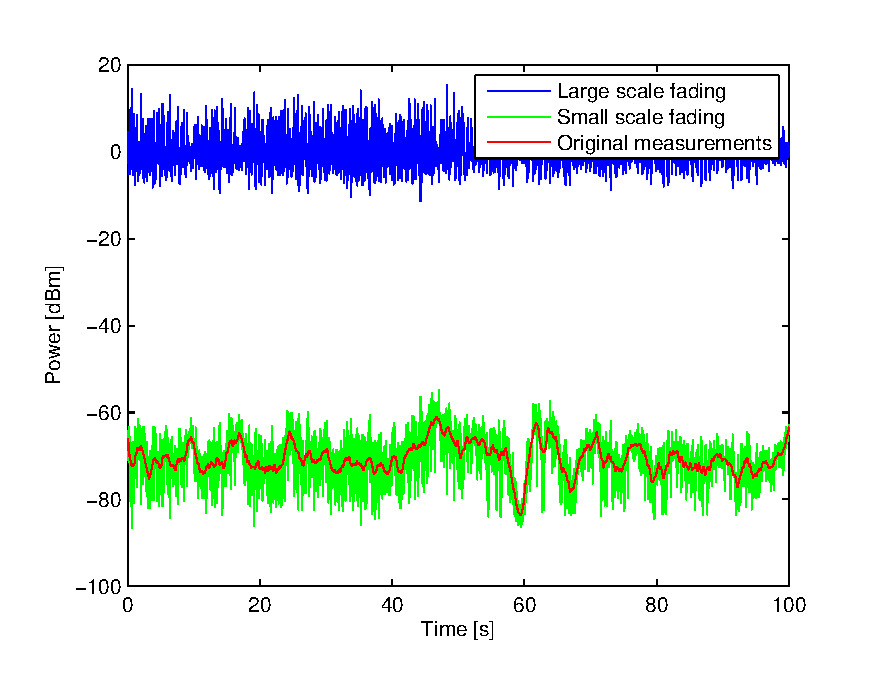
\includegraphics[width=1.0\textwidth]{task1.eps}
    \caption{Large scale, small scale and original measurements of data}
    \label{fig:task1}
\end{figure}

\section{Task 2}

\begin{figure}[H]
    \centering
    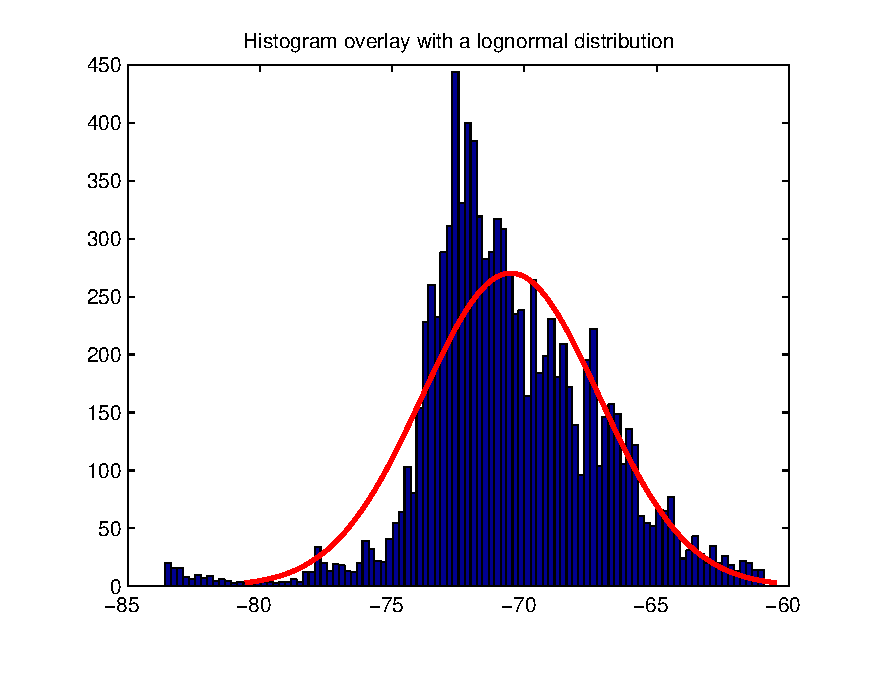
\includegraphics[width=1.0\textwidth]{task2.eps}
    \caption{Histogram of large scale fading.}
    \label{fig:task2}
\end{figure}





\end{document}



